\documentclass[12pt]{amsart}
\usepackage{fullpage}
\usepackage{pbox}
\usepackage{graphicx}
\usepackage{booktabs} % Top and bottom rules for table
\usepackage{amsfonts, amsmath, amsthm, amssymb}
\usepackage{longtable,array,color,xcolor}
\usepackage[colorlinks = true,
            urlcolor  = blue]{hyperref}
\usepackage{verbatim}
\usepackage{enumerate}
\newcommand\narrowstyle{\SetTracking{encoding=*}{-50}\lsstyle}

\setlength{\parindent}{0pt}

\begin{document}
\flushright
Name:\underline{\hspace{5cm}}
\title{Math 320: Quiz 2}
\maketitle

\begin{enumerate}
\item (3 points) Let $f(x) = x^3-7$. Suppose we would
like to find a root of $f(x)$ in the interval $(0,2)$ using the
two endpoints as our ``bracket.''

\begin{enumerate}
\item What are the first two points selected inside the 
interval using the bisection method? Justify your response.

\item How many iterations of the bisection method must be performed
to guarantee error less than $2^{-16}$?

\item What is the first point in the interval selected by
the false position (regula falsi) method?
\end{enumerate}

\vfill
\pagebreak

\item (3 points) Let $f(x) = (x^2-1)e^{-x^2}$ be our function of
interest, with graph shown below. 

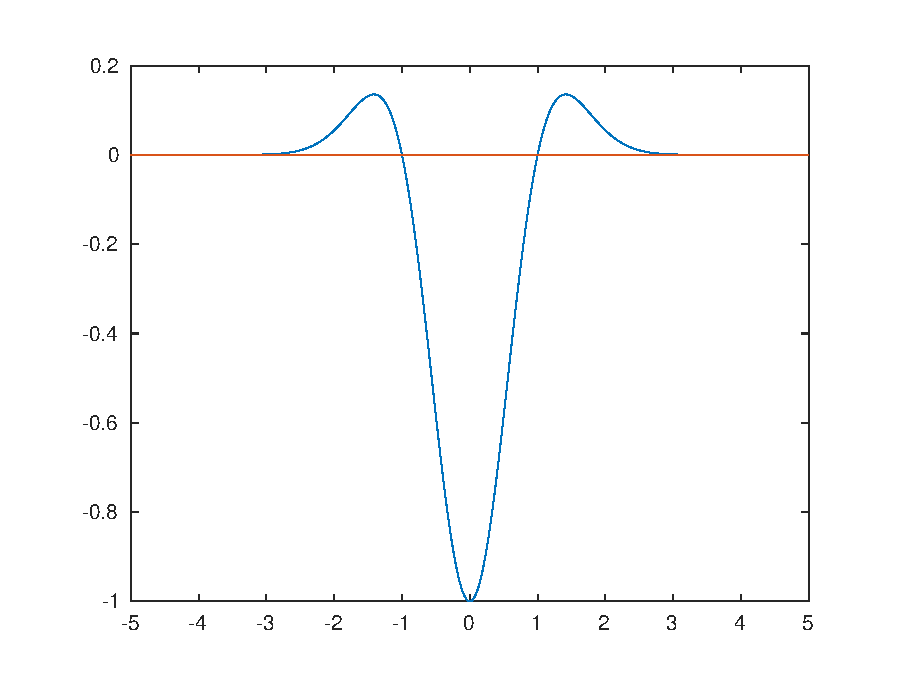
\includegraphics{q3p2.eps}
Suppose we try to find a root using Newton's method.

\begin{enumerate}
\item 

\item Evaluate the $n$-th order approximation to $10.1^{10}$ for
$n = 0,1$, and $2$.


\item Compute the approximate relative error in the 
first-order approximation.


\item To one significant digit, what is the approximate relative error
in the second-order approximation?



\end{enumerate}


\end{enumerate}
\end{document}
